\documentclass[twocolumn,a4j]{jarticle}
\usepackage[dvipdfmx]{graphicx}
\usepackage{url}
\usepackage{ascmac}
\usepackage{amsmath}
\usepackage{fancyhdr}


% 所属と氏名を右寄せにする設定
\makeatletter
  \def\@maketitle{%
  \newpage\null
  %\vskip 2em%
  \begin{center}%
  \let\footnote\thanks
    {\LARGE \@title \par}%
    %\vskip 1.5em%
  \end{center}% 追加
    \mbox{}\hfill%% 追加
    {\large
      %\lineskip .5em%
      \begin{tabular}[t]{c}%
        \@author
      \end{tabular}\par}%
    \vskip 1em%
  \begin{center}% 追加
    {\large \@date}%
  \end{center}%
  %\par\vskip 1.5em
}

% section前後の行間を詰める設定
\renewcommand{\section}{\@startsection{section}{1}{\z@}%
   {.3\Cvs \@plus.5\Cvs \@minus.2\Cvs}% % section上部の空白量
   {.2\Cvs \@plus.3\Cvs}%                % section下部の空白量
   {\reset@font\Large\bfseries}}         % フォント,フォントサイズを変更
\renewcommand{\subsection}{\@startsection{subsection}{2}{\z@}%
   {.3\Cvs \@plus.5\Cvs \@minus.2\Cvs}%
   {.2\Cvs \@plus.3\Cvs}%
   {\reset@font\large\bfseries}}
\renewcommand{\subsubsection}{\@startsection{subsubsection}{3}{\z@}%
   {.3\Cvs \@plus.5\Cvs \@minus.2\Cvs}% 
   {.2\Cvs \@plus.3\Cvs}%
   {\reset@font\normalsize\bfseries}}

\makeatother


% 余白の設定
\usepackage[top=20truemm,bottom=20truemm,left=20truemm,right=20truemm]{geometry}


%%%%%%%%%%%%%%%%%%%%%%%%%%%%%%%% 皆さんが書き換えるのはここから %%%%%%%%%%%%%%%%%%%%%%%%%%%%%%%%%%%%%%%

\title{\TeX を使おう!\\		% タイトル
{\small 金子・中村研ゼミ資料}	% 出展
}
\author{知能機械工学科 金子・中村研究室\\123456 中村友昭} % 所属,学籍番号,名前
\date{}


%%%%%%%%%%%%%%% 練習7 %%%%%%%%%%%%%%%%%
% ここの数字をいじってページ数をちょうど4ページに合わせてみましょう.
\renewcommand{\baselinestretch}{1.0}
%%%%%%%%%%%%%%% ここまで %%%%%%%%%%%%%%%%%


\begin{document}
\maketitle

\renewcommand{\headrulewidth}{0.0pt}
\thispagestyle{fancy}
\lhead{}
\rhead{輪講報告 2015/7/26提出}
\cfoot{\thepage{}}

\def\bq{\begin{equation}}
\def\eq{\end{equation}}
\def\beq{\begin{eqnarray}}
\def\eeq{\end{eqnarray}}
\def\ba{\begin{array}}
\def\ea{\end{array}}
\def\bc{\begin{center}}
\def\ec{\end{center}}

\def\dsum{\sum\limits}
\def\disp{\displaystyle}
\def\ejw{e^{j\omega}}
\def\ejwi{e^{j\omega_{i}}}
\def\e-jwi{e^{-j\omega_{i}}}
\def\dfrac#1#2{\disp{\frac{#1}{#2}}}
\def\teigi{\stackrel{\triangle}{=}}


%\def\b0{\mbox{\boldmath$0$}}


\if0
\def\baa{\mbox{\boldmath$a$}}
\def\bb{\mbox{\boldmath$b$}}
\def\bcc{\mbox{\boldmath$c$}}
\def\bd{\mbox{\boldmath$d$}}
\def\be{\mbox{\boldmath$e$}}
\def\bff{\mbox{\boldmath$f$}}
\def\bg{\mbox{\boldmath$g$}}
\def\bh{\mbox{\boldmath$h$}}
\def\bi{\mbox{\boldmath$i$}}
\def\bj{\mbox{\boldmath$j$}}
\def\bk{\mbox{\boldmath$k$}}
\def\bl{\mbox{\boldmath$l$}}
\def\bm{\mbox{\boldmath$m$}}
\def\bn{\mbox{\boldmath$n$}}
\def\bo{\mbox{\boldmath$o$}}
\def\bp{\mbox{\boldmath$p$}}
\def\bqq{\mbox{\boldmath$q$}}
\def\br{\mbox{\boldmath$r$}}
\def\bs{\mbox{\boldmath$s$}}
\def\bt{\mbox{\boldmath$t$}}
\def\bu{\mbox{\boldmath$u$}}
\def\bv{\mbox{\boldmath$v$}}
\def\bw{\mbox{\boldmath$w$}}
\def\bx{\mbox{\boldmath$x$}}
\def\by{\mbox{\boldmath$y$}}
\def\bz{\mbox{\boldmath$z$}}

\def\bA{\mbox{\boldmath$A$}}
\def\bB{\mbox{\boldmath$B$}}
\def\bC{\mbox{\boldmath$C$}}
\def\bD{\mbox{\boldmath$D$}}
\def\bE{\mbox{\boldmath$E$}}
\def\bF{\mbox{\boldmath$F$}}
\def\bG{\mbox{\boldmath$G$}}
\def\bH{\mbox{\boldmath$H$}}
\def\bI{\mbox{\boldmath$I$}}
\def\bJ{\mbox{\boldmath$J$}}
\def\bK{\mbox{\boldmath$K$}}
\def\bL{\mbox{\boldmath$L$}}
\def\bM{\mbox{\boldmath$M$}}
\def\bN{\mbox{\boldmath$N$}}
\def\bO{\mbox{\boldmath$O$}}
\def\bP{\mbox{\boldmath$P$}}
\def\bQ{\mbox{\boldmath$Q$}}
\def\bR{\mbox{\boldmath$R$}}
\def\bS{\mbox{\boldmath$S$}}
\def\bT{\mbox{\boldmath$T$}}
\def\bU{\mbox{\boldmath$U$}}
\def\bV{\mbox{\boldmath$V$}}
\def\bW{\mbox{\boldmath$W$}}
\def\bX{\mbox{\boldmath$X$}}
\def\bY{\mbox{\boldmath$Y$}}
\def\bZ{\mbox{\boldmath$Z$}}
\fi



\if0
\def\b0{\bf{0}}
\def\bPhi{\mbox{\boldmath$\Phi$}}
\def\bomega{\mbox{\boldmath$\omega$}}
\def\bLambda{\mbox{\boldmath$\Lambda$}}
\def\blambda{\mbox{\boldmath$\lambda$}}
\def\bmu{\mbox{\boldmath$\mu$}}
\def\bnu{\mbox{\boldmath$\nu$}}
\def\bSigma{\mbox{\boldmath$\Sigma$}}
\def\bPhi{\mbox{\boldmath$\Phi$}}
\def\balpha{\mbox{\boldmath$\alpha$}}
\def\bTheta{\mbox{\boldmath$\Theta$}}
\def\btheta{\mbox{\boldmath$\theta$}}
\def\bGamma{\mbox{\boldmath$\Gamma$}}
\def\bPsi{\mbox{\boldmath$\Psi$}}
\def\bDelta{\mbox{\boldmath$\Delta$}}
\def\bPi{\mbox{\boldmath$\Pi$}}
\fi

\makeatletter
\def\lddots{\mathinner{\mkern1mu\raise\p@\vbox{\kern7\p@\hbox{.}}\mkern2mu
\raise4\p@\hbox{.}\mkern2mu\raise7\p@\hbox{.}\mkern1mu}}
\makeatother


\def\argmax{\mathop{\rm argmax}}




\def\baa{{ \boldsymbol a}}
\def\bb{{ \boldsymbol b}}
\def\bcc{{ \boldsymbol c}}
\def\bd{{ \boldsymbol d}}
\def\be{{ \boldsymbol e}}
\def\boldsymbolf{{ \boldsymbol f}}
\def\bg{{ \boldsymbol g}}
\def\bh{{ \boldsymbol h}}
\def\bi{{ \boldsymbol i}}
\def\bj{{ \boldsymbol j}}
\def\bk{{ \boldsymbol k}}
\def\bl{{ \boldsymbol l}}
\def\bm{{ \boldsymbol m}}
\def\bn{{ \boldsymbol n}}
\def\bo{{ \boldsymbol o}}
\def\bp{{ \boldsymbol p}}
\def\bqq{{ \boldsymbol q}}
\def\br{{ \boldsymbol r}}
\def\bs{{ \boldsymbol s}}
\def\bt{{ \boldsymbol t}}
\def\bu{{ \boldsymbol u}}
\def\bv{{ \boldsymbol v}}
\def\bw{{ \boldsymbol w}}
\def\bx{{ \boldsymbol x}}
\def\by{{ \boldsymbol y}}
\def\bz{{ \boldsymbol z}}

\def\bA{{ \boldsymbol A}}
\def\bB{{ \boldsymbol B}}
\def\bC{{ \boldsymbol C}}
\def\bD{{ \boldsymbol D}}
\def\bE{{ \boldsymbol E}}
\def\bF{{ \boldsymbol F}}
\def\bG{{ \boldsymbol G}}
\def\bH{{ \boldsymbol H}}
\def\bI{{ \boldsymbol I}}
\def\bJ{{ \boldsymbol J}}
\def\bK{{ \boldsymbol K}}
\def\bL{{ \boldsymbol L}}
\def\bM{{ \boldsymbol M}}
\def\bN{{ \boldsymbol N}}
\def\bO{{ \boldsymbol O}}
\def\bP{{ \boldsymbol P}}
\def\bQ{{ \boldsymbol Q}}
\def\bR{{ \boldsymbol R}}
\def\bS{{ \boldsymbol S}}
\def\bT{{ \boldsymbol T}}
\def\bU{{ \boldsymbol U}}
\def\bV{{ \boldsymbol V}}
\def\bW{{ \boldsymbol W}}
\def\bX{{ \boldsymbol X}}
\def\bY{{ \boldsymbol Y}}
\def\bZ{{ \boldsymbol Z}}


\def\b0{{\boldsymbol 0}}
\def\bPhi{{\boldsymbol\Phi}}
\def\bomega{{\boldsymbol\omega}}
\def\bLambda{{\boldsymbol\Lambda}}
\def\blambda{{\boldsymbol\lambda}}
\def\bmu{{\boldsymbol\mu}}
\def\bnu{{\boldsymbol\nu}}
\def\bSigma{{\boldsymbol\Sigma}}
\def\bPhi{{\boldsymbol\Phi}}
\def\balpha{{\boldsymbol\alpha}}
\def\bTheta{{\boldsymbol\Theta}}
\def\btheta{{\boldsymbol\theta}}
\def\bGamma{{\boldsymbol\Gamma}}
\def\bPsi{{\boldsymbol\Psi}}
\def\bDelta{{\boldsymbol\Delta}}
\def\bPi{{\boldsymbol\Pi}}


\section{はじめに}
TeXは皆さんが思っているほど難しいものではありません.
コマンドを覚えなければいけないと思っているかもしれませんが,
基本はwebからのコピペや,過去作った文書からのコピペでなんとかなります.
TeXは,論文やこの原稿のような文書を作成するのに最適化されています.
Wordは様々な``おせっかい''な機能のため図の配置が意図しない場所に移動してしまうことがありますが,
TeXでは論文のスタイルに沿った最適な位置へ配置をしてくれます.
(もちろん,Wordと違い簡単に思った位置に図を配置することもできます.)
さらに,論文に必要な図のキャプションや数式番号,参考文献番号などもWordに比べて簡単に管理することができます.
(Wordでは思い通りの番号が付かないこともあります.)

以上のような理由から,初学者がWordとTeXで原稿を作った場合には,
圧倒的にTeXで作ったものの方が論文のスタイルに沿ったものができ,完成度が高くなります
\footnote{全てに関してTeXがいいというわけではなく,書式が自由な簡単な文書であればWordの方が簡単です.適材適所で使い分けるといいと思います.(TeXであればこんな注釈も簡単に出せます.)}.
使ってみると論文を書くことに関しては圧倒的にTeXの方が簡単なので,是非集中輪講を機に挑戦してください.


\section{ \TeX のインストール}
ホームページ\cite{tex}から,インストーラをダウンロードして,実行すると依存ファイルも含めてインストールできます.
基本的には「次へ」を押すだけです.
このインストーラでは,texworksというTeXの統合環境もインストールされます.
早速,texworksを起動してこの文書のソースファイルmain.texを開いてみましょう.
ソースの最上部には色々難しそうなものが書いてありますが,皆さんがここを書き換える必要はありません.
「\%\% 皆さんが書き換えるのはここから \%\%」と書いてある行以降を書き換えます.

コンパイルは左上の再生ボタン(っぽい形のボタン)を押すとコンパイルされて,PDFが作成されます.
もし,参考文献や数式の参照が[?]になっていたら,もう一度コンパイルしてみてください.

\section{章の作り方}
章,節,項は\verb|\section{章},\subsection{節},\subsubsection{項}|と記述すると作成することができます.
実際の出力結果が次章です.

\section{章}
\subsection{節}
\subsubsection{項}
\subsection{練習1}
ソースを書き換えて新たな5章を作ってみましょう.章が作られ番号が自動的に振られるのが分かるかと思います.

%%%%%%%%%%%%%%%%%%% 練習1 %%%%%%%%%%%%%%%%%%%%%
% ここに独自の章を作ってみましょう.
% コマンドはコピペしましょう


%%%%%%%%%%%%%%%%%% ここまで %%%%%%%%%%%%%%%%%%%%%


\section{参考文献の書き方}
参考文献は,以下のような書式で,文書の下の方に書きます.
\begin{screen}
\verb|\bibitem{nakamura2014}|\\
\verb|中村友昭,|\\
\verb|``\TeX を使おう!'', |\\
\verb|ゼミ資料, pp.1-5, 2014|
\end{screen}
参照は\verb|\cite{nakamura2014}|と書くと,\cite{nakamura2014}のように自動的に番号を振ってくれます.

\subsection{練習2}
この文書のソースファイルに,新たな参考文献を追加して,その参考文献への参照を追加しましょう.
番号が[?]になったり,ずれる場合は,再度コンパイルすると治ります.

%%%%%%%%%%%%%%% 練習2 %%%%%%%%%%%%%%%%%
% 独自の参考文献を追加してみましょう(このファイルの下部)
% 独自に追加した参考文献を参照してみましょう
% 例: これ\cite{aaaa}が独自に追加した参考文献である.


%%%%%%%%%%%%%%% ここまで %%%%%%%%%%%%%%%%%

\section{箇条書き}
箇条書きにはいくつか種類があり,それぞれ以下のように記述します.

\subsection{箇条書き1}
\begin{screen}
\verb|\begin{itemize}|\\
\verb|\item 普通の箇条書き|\\
\verb|\item 項目を増やすにはitemを追加する|\\
\verb|\end{itemize}|
\end{screen}
%
出力は次のようになります.
%
\begin{itemize}
 \item 普通の箇条書き
 \item 項目を増やすにはitemを追加する
\end{itemize}

\subsection{箇条書き2}
\begin{screen}
\verb|\begin{enumerate}|\\
\verb|\item 番号付きの箇条書き|\\
\verb|\item 項目を増やすにはitemを追加する|\\
\verb|\end{enumerate}|
\end{screen}
%
出力は次のようになります.
%
\begin{enumerate}
 \item 番号付きの箇条書き
 \item 項目を増やすにはitemを追加する
\end{enumerate}

\subsection{箇条書き}
\begin{screen}
\verb|\begin{description}|\\
\verb|\item[項目A] 項目名付きの箇条書き|\\
\verb|\item[項目B] 項目を増やすにはitemを追加|\\
\verb|\end{description}|
\end{screen}
%
出力は次のようになります.
%
\begin{description}
 \item[項目A] 項目名付きの箇条書き
 \item[項目B] 項目を増やすにはitemを追加
\end{description}


\subsection{練習3}
ソースファイルを編集して,ここにあなたの好きな食べ物トップ5を箇条書きで書いてみましょう.
箇条書きの種類はどれを使っても構いません.

%%%%%%%%%%%%%%% 練習3 %%%%%%%%%%%%%%%%%
% 箇条書きで好きな食べ物トップ5を書いてみよう.


%%%%%%%%%%%%%%% ここまで %%%%%%%%%%%%%%%%%






\section{図の挿入}
\subsection{図の作成方法}

\begin{figure}[t]
  \centering
  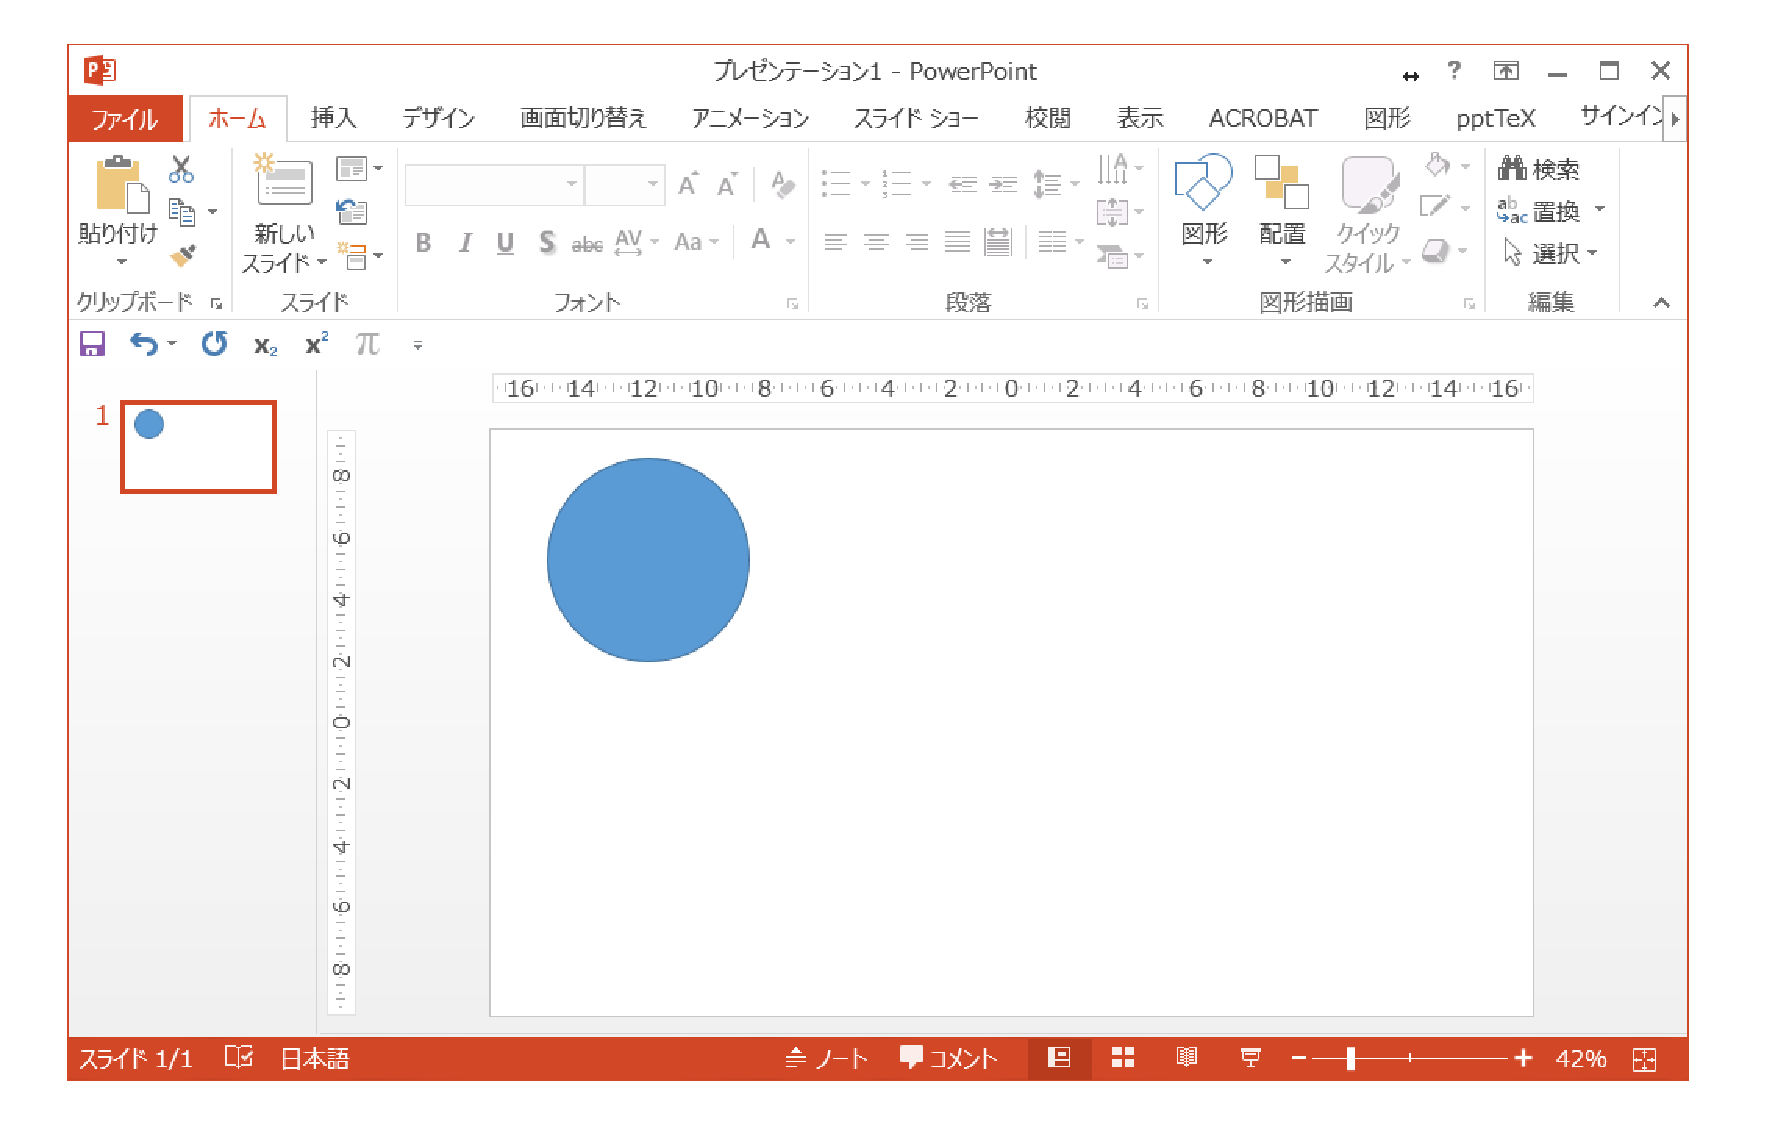
\includegraphics[scale=0.3]{fig/make_fig.pdf}
  \caption{パワーポイントによる図の作成}
  \label{fig:make_fig}
\end{figure}

\begin{figure}[t]
  \centering  
  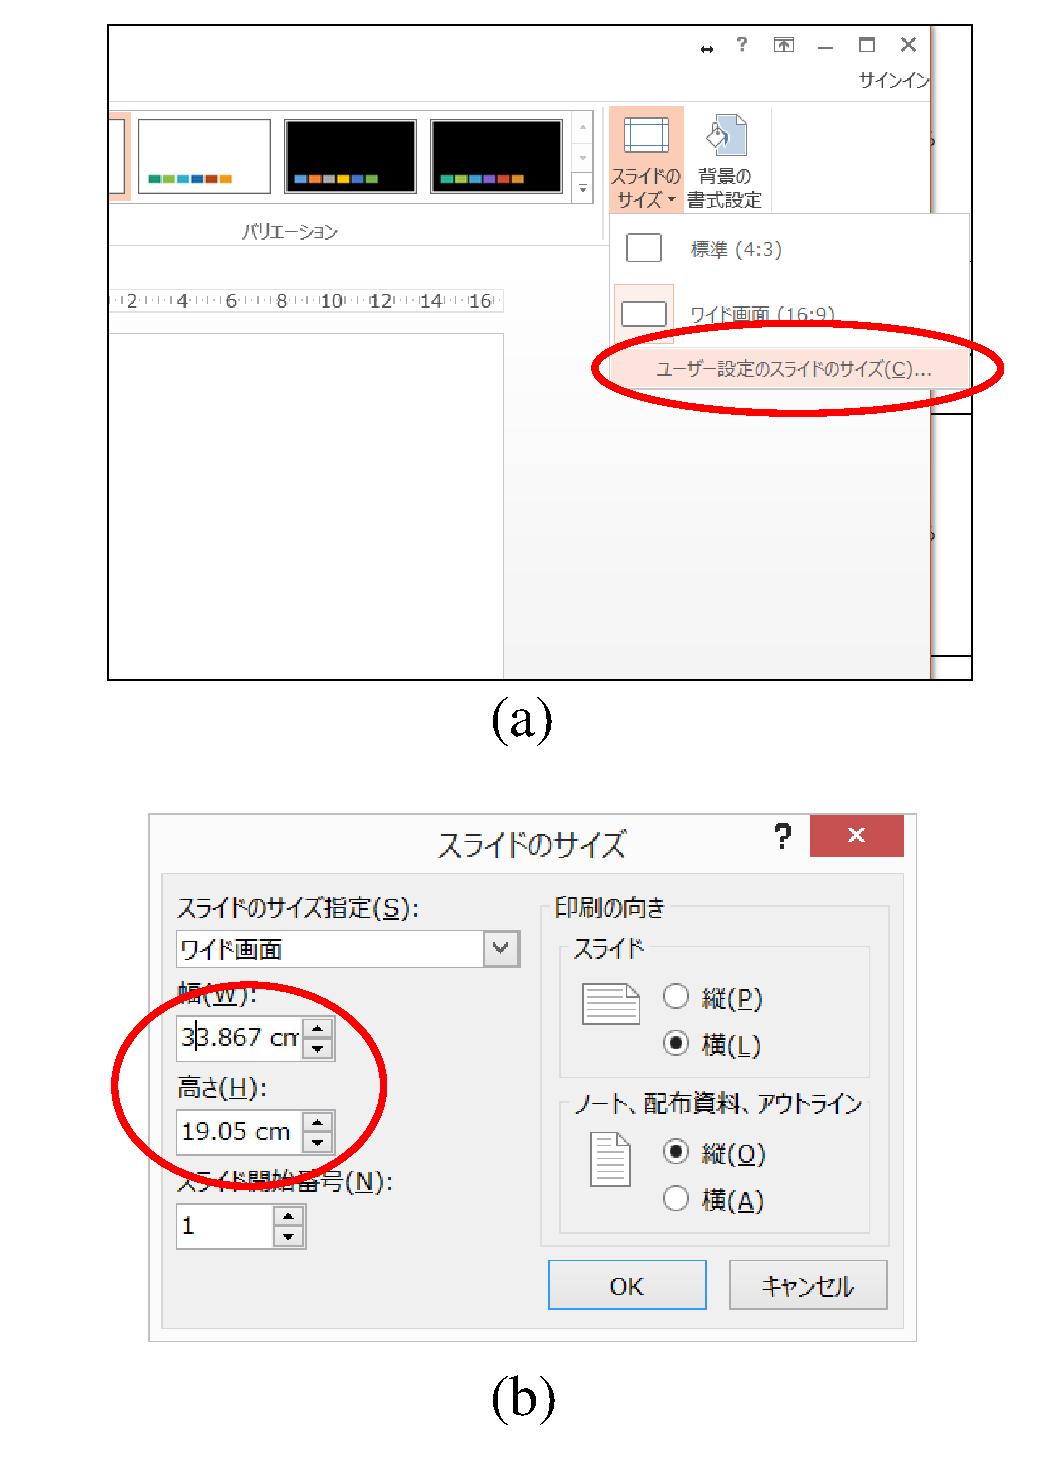
\includegraphics[scale=0.4]{fig/trim_fig.pdf}
  \caption{余白の削除~~(a)スライドのサイズ変更ダイアログの起動~~(b)スライドのサイズの変更}
  \label{fig:trim_fig}
\end{figure}

\begin{figure}[t]
  \centering
  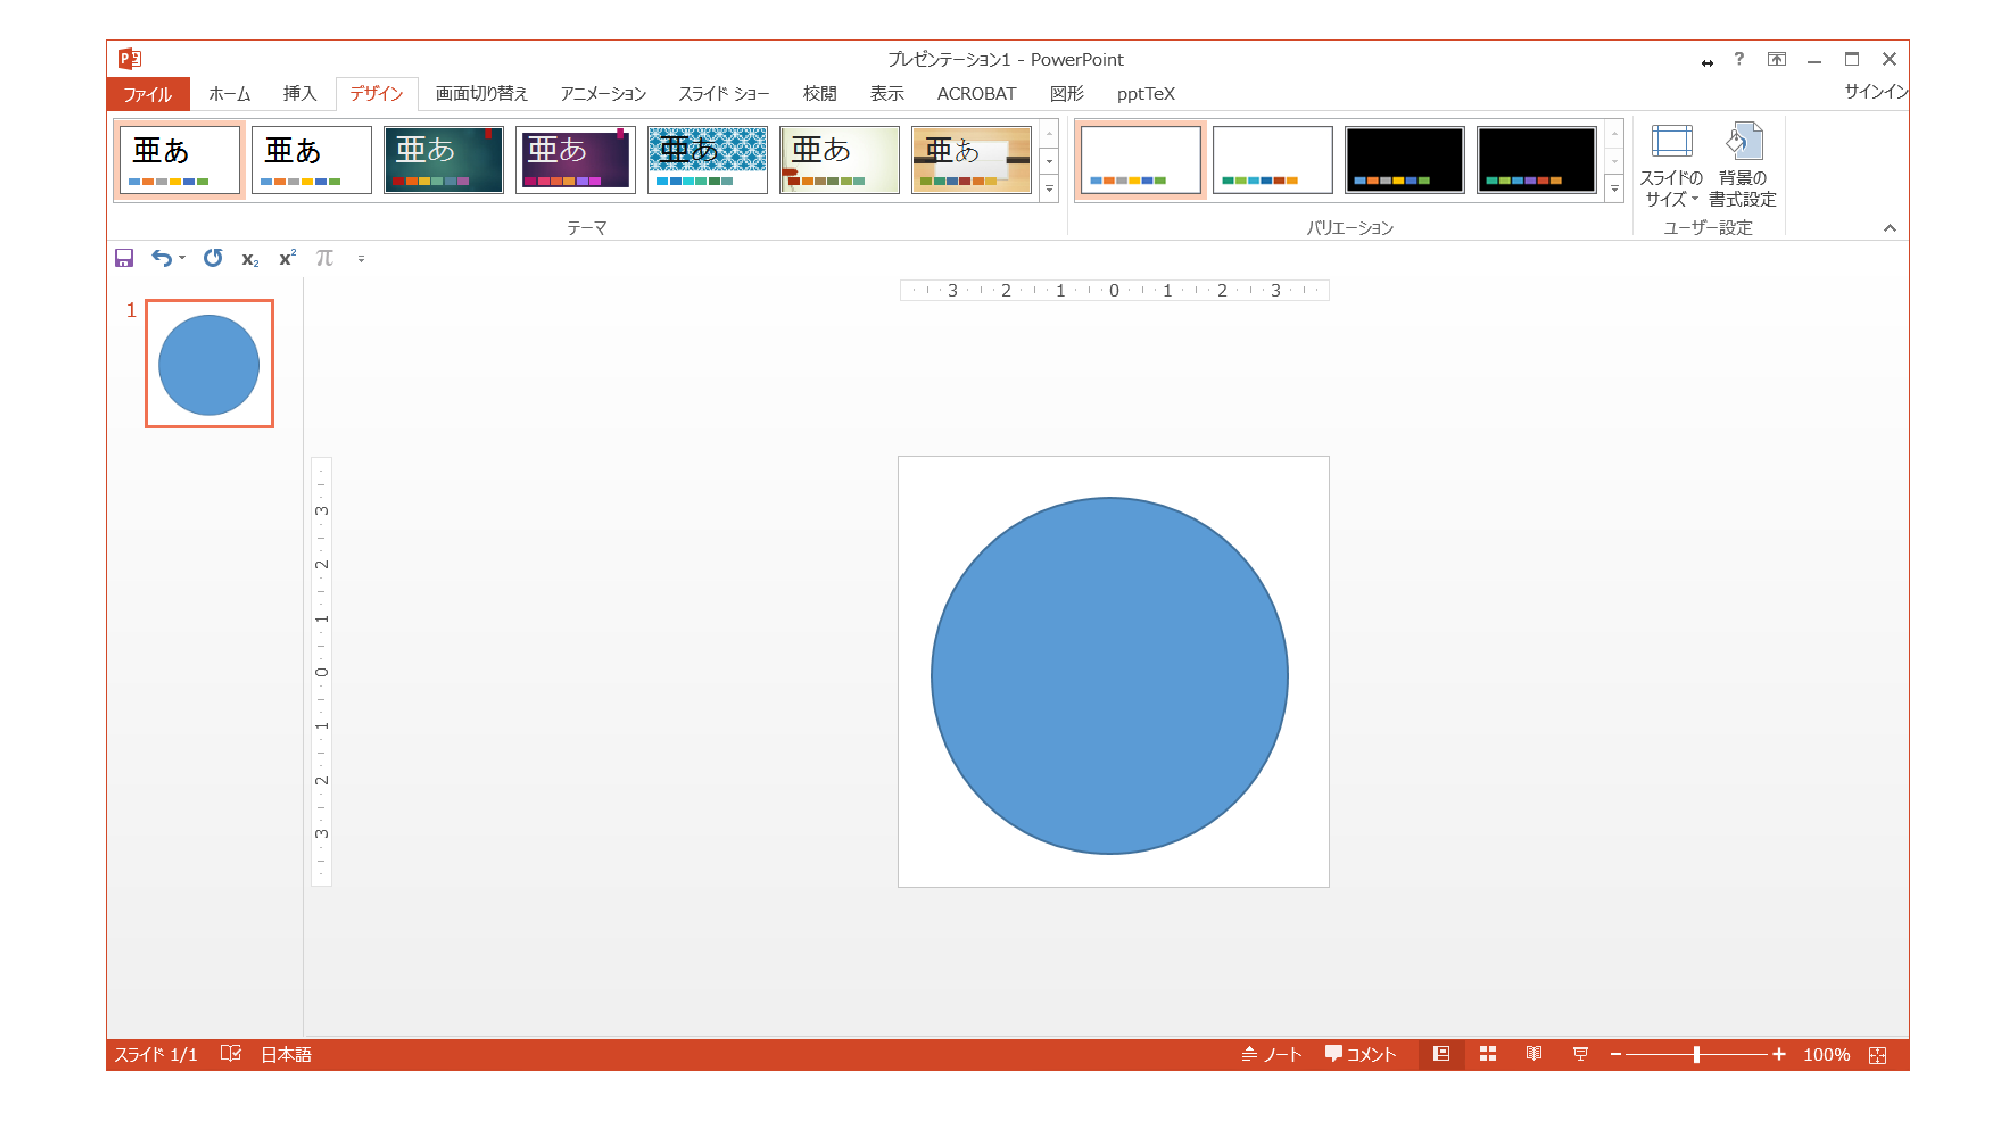
\includegraphics[scale=0.25]{fig/trim_fig2.pdf}
  \caption{余白が削除されたパワーポイント}
  \label{fig:trim_fig2}
\end{figure}

\begin{figure}[t]
 \centering 
  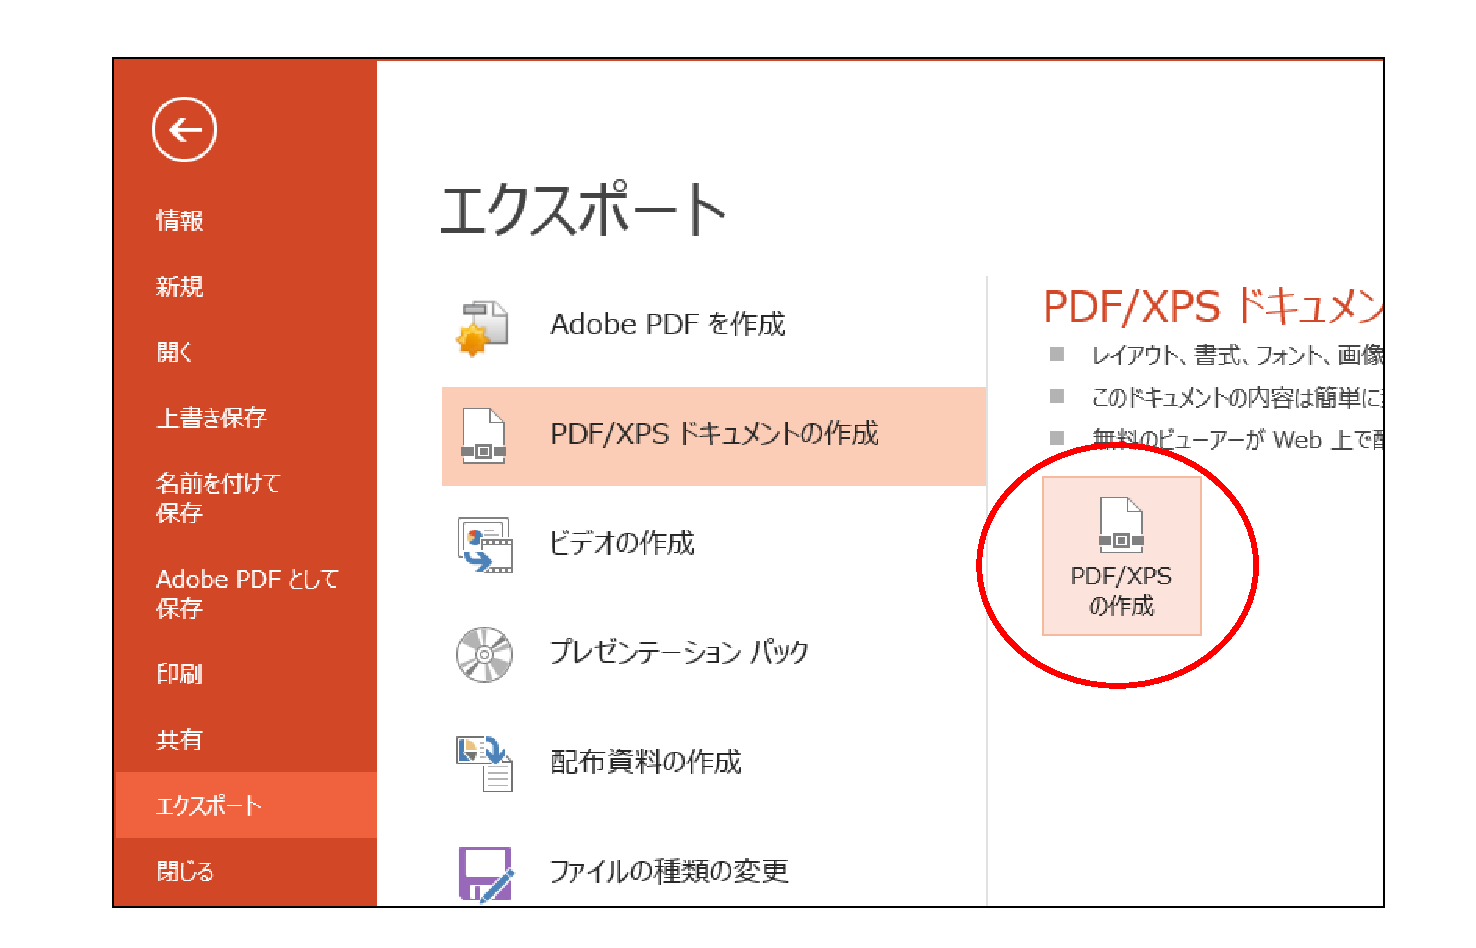
\includegraphics[scale=0.25]{fig/save_pdf.pdf}
  \caption{図の保存}
  \label{fig:save_fig}
\end{figure}

\begin{figure}[t]
 \centering 
  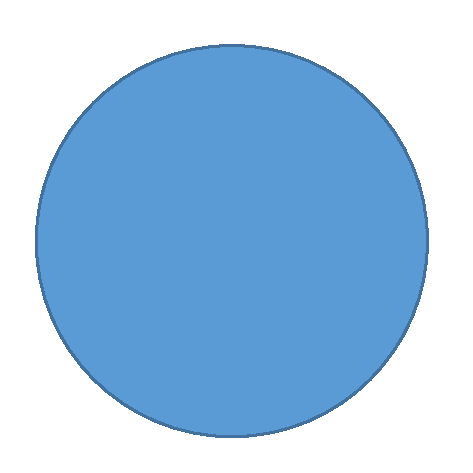
\includegraphics[scale=0.25]{fig/fig.pdf}
  \caption{挿入された図}
  \label{fig:circle}
\end{figure}



TeXで最も面倒なのが図の作成です.TeXではpdfやepsという形式の図のみ挿入可能です.
ここでは,パワーポイントの標準機能を使ってPDFで画像を作る方法を紹介します.
まず,図\ref{fig:trim_fig}のように1枚のスライドのみで構成されたパワーポイントで画像を作成します.
しかし,このまま出力するとスライドの白い領域が余白として,そのまま出力されてしまいます.
そこで,スライドのサイズを変更して余白を削除します.
まず,図\ref{fig:trim_fig}(a)のように以下のパワーポイントのメニューを辿っていき,スライドのサイズ変更ダイアログ(図\ref{fig:trim_fig}(b))を起動します.
%
\begin{center}
[デザイン]タブ

↓

[スライドのサイズ]

↓

[ユーザー設定のスライドのサイズ]
\end{center}
%
このダイアログ(図\ref{fig:trim_fig}(b))に適当な数字を入力しスライドの余白をなくし,図\ref{fig:trim_fig2}のような無駄な余白がない状態にします.
最後に,図\ref{fig:save_fig}のように以下のメニューを辿っていき,PDFとして画像を保存します.
%
\begin{center}
[ファイル]

↓

[エクスポート]

↓

[PDF/XPSドキュメントの作成]

↓

[PDF/XPSの作成]
\end{center}
%
元画像のPPTXのファイル名は何でも構いませんが,PDFファイルと同名にし,PDFファイルと同一ディレクトリに入れておくと,
編集をする際に便利です.
このTEXサンプルでは,figフォルダにPPTXとPDFの両方を入れてあります.

\subsection{図の挿入}
図は次のようなコマンドで挿入できます.
%
\begin{screen}
\verb|\begin{figure}[t]|\\
\verb|\centering|\\
\verb|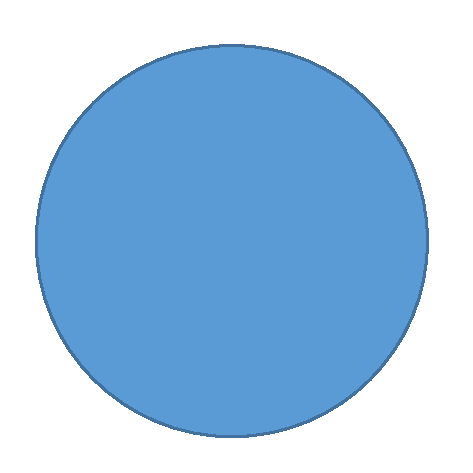
\includegraphics[scale=0.25]{fig/fig.pdf}|\\
\verb|\caption{挿入された図}|\\
\verb|\label{fig:circle}|\\
\verb|\end{figure}|
\verb|\end{description}|
\end{screen}
%
この結果,表示された図が図\ref{fig:circle}になります.
このコマンドは非常に長いですが,覚える必要はありません.
必要なときにコピペを利用してください.
その際に,必要に応じて以下の場所を変更してください.
まず,3行目の\verb|\includegraphics|では,1つ目の引数のscaleに指定されている数字(0.25)が図の大きさで,
2つ目の引数(\verb|fig/fig.pdf|)がpdfファイルのファイル名です.
 \verb|\caption|は図のキャプション(タイトル)なので,好きな文字列に変更してください.
また,\verb|\label|は図を参照するときに必要なラベルになります.
本文中に「\verb|図\ref{fig:circle}|」と書くことで「図\ref{fig:circle}」のように,図を参照することができます.
なので,ラベルは他の図とはかぶらない分かりやすい名前にした方がいいです.

\subsection{練習4}
figフォルダ内にパワーポイントで画像を作成して,ここに挿入してみましょう.
また,その図を参照するような本文を書いてみましょう.

%%%%%%%%%%%%%%% 練習4 %%%%%%%%%%%%%%%%%
% 1,figフォルダ内にパワーポイントファイルを作成
% 2,図をパワーポイントで作成
% 3,その図をpdfへ変換
% 4,図の挿入コマンドをコピペして,必要な箇所を変更
% 5,図を参照するような本文を追加してみましょう
%     例:図\ref{***}が新たに追加した図である.




%%%%%%%%%%%%%%% ここまで %%%%%%%%%%%%%%%%%



\section{表の挿入}
表は次のコマンドで挿入できます.
%
\begin{screen}
\verb|\begin{table}[t]|\\
\verb|\caption{簡単な表の挿入}|\\
\verb|\label{tbl:example}|\\
\verb|\centering|\\
\verb+\begin{tabular}{|c||c|c|} \hline+\\
\verb|名前 &  学籍番号 & 出身地 \\ \hline \hline|\\
\verb|太郎 &  999 & 東京 \\ \hline|\\
\verb|花小 &  777 & 埼玉 \\ \hline|\\
\verb|\end{tabular}|\\
\verb|\end{table}|
\end{screen}
%
\begin{table}[t]
 \caption{簡単な表の挿入}
 \label{tbl:example}
 \centering
  \begin{tabular}{|c||c|c|} \hline
   名前 &  学籍番号 & 出身地 \\ \hline \hline
   太郎 &  999 & 東京 \\ \hline
   花小 &  777 & 埼玉 \\ \hline
  \end{tabular}
\end{table}
%
その結果が表\ref{tbl:example}です.
これも図の挿入と同様に,コマンドを覚える必要はなく,コピペをし必要な箇所を各自で修正をしてください.
\verb|\caption|と\verb|\label|は,図の場合と同様に,それぞれ表のキャプション(タイトル)と表を参照するためのラベルです.
\verb+\begin{tabular}{|c||c|c|}+の「\verb+|c||c|c|+」は,「\verb+|+」が縦線を,「c」が各項目の配置を表しています.
「\verb+|c|+」は各項目を中心(center)に寄せて表示し,その両側に縦線を引くことを意味しています.
また,「\verb+||+」は二重線を意味しています.
配置は,「c」以外にも,「l」(left:左寄せ)や「r」(right:右寄せ)が利用できます.

「\verb|太郎 &  999 & 東京 \\ \hline|」では,「\&」は項目の区切りを表し,「\verb|\\|」は行の終わりを,「\verb|\hline|」は横線を挿入することをそれぞれ意味しています.
横線も縦線と同様に二重線にすることができ,「\verb|\hline \hline|」と2つ記述することで二重線になります.

行を追加したい場合は,該当箇所に例えば「\verb|次郎 &  666 & 栃木 \\ \hline|」といった行を挿入します.
列を追加したい場合は多少面倒ですが,「\verb+\begin{tabular}{|c||c|c|c|} \hline+」のように「\verb+c|+」を追加し,
「\verb|名前 &  学籍番号 & 出身地 & 年齢 \\ \hline \hline|」のように,各行に項目を追加します.

\subsection{練習5}
$4 \times 4$の表を作ってみましょう.また,その表を参照するような本文をここに書いてみましょう.

%%%%%%%%%%%%%%% 練習5 %%%%%%%%%%%%%%%%%
% 1,表を作成する
% 2,本文を参照するような本文を記述する
%     例:表\ref{***}が新たに追加した表である.




%%%%%%%%%%%%%%% ここまで %%%%%%%%%%%%%%%%%


\section{数式}
TeXの強みは数式を簡単にきれいに出力できる点です.
本文中の数式は「\$」と「\$」ではさみ,「\verb|$a \times b$|」と記述することで,
$a \times b$のように出力することができます.
別の行に数式を書きたいときは,以下のように記述します.
\begin{screen}
\verb|\begin{eqnarray}|\\
\verb|x^2 - 6x_1 + 1 &=& 0 \label{eq:example} \\|\\
\verb|y &=& a x + b|\\
\verb|\end{eqnarray}|
\end{screen}
%
その結果が以下となります.
%
\begin{eqnarray}
  x^2 - 6x_1 + 1 &=& 0 \label{eq:example} \\
  y &=& a x + b
\end{eqnarray}
%
「\verb|\label{eq:example}|」はなくても構いません.
図や表と同様に本文で参照する場合のみ利用し,「\verb|式(\ref{eq:example})|」と記述することで,
式(\ref{eq:example})のように参照することができます.
「\verb|\\|」は改行を表しており,複数行の数式を書くことができます.
その際,「\verb|&|」と「\verb|&|」に囲まれた文字(この例だと「$=$」)が同じ位置にくるように自動的に調整されます.


\begin{table}[t]
 \caption{数式の特殊な記法}
 \label{tbl:mathsign}
  \centering
  \begin{tabular}{|c||c|c|} \hline
   コマンド & 出力 & 説明 \\ \hline \hline
   \verb|a^b| &  $a^b $ & 上付き文字 \\ \hline
   \verb|a_b| &  $a_b $ & 下付き文字 \\ \hline
   \verb|\frac{a}{b}| &  $\frac{a}{b}$ & 分数 \\ \hline
   \verb|a \times b| &  $a \times b$ & 掛け算 \\ \hline
   \verb|a \propto b| &  $a \propto b$ & 比例 \\ \hline
   \verb|a \neq b| &  $a \neq b$ & 不等 \\ \hline
   \verb|a \geq b | &  $ a \geq b $ & 不等号\footnotemark[2] \\ \hline
   \verb|a \leq b | &  $ a \leq b $ & 不等号 \\ \hline
   \verb| \baa, \bb, \bcc, \bd | &  $\baa, \bb, \bcc, \bd$ & 太字\footnotemark[3] \\ \hline
   \verb|\sin| &  $ \sin $ & sin関数 \\ \hline
   \verb|\cos| &  $ \cos $ &cos関数 \\ \hline
   \verb|\tan| &  $ \tan $ & tan関数 \\ \hline
   \verb|\log| &  $ \log $ & log関数 \\ \hline
   \verb|\int_a^b| &  $ \int_a^b $ & 積分 \\ \hline
  \end{tabular}
\end{table}

\footnotetext[2]{=なしの不等号は「$<$」「$>$」をそのまま入力}
\footnotetext[3]{上部で$\backslash$input\{contents\}をする必要がある} 

\begin{table}[t]
 \caption{ギリシャ文字}
 \label{tbl:mathchar}
 \begin{center}
  \begin{tabular}{|c|c||c|c|} \hline
   コマンド & 出力 & コマンド & 出力 \\ \hline \hline
  \verb|\alpha| & $\alpha$ & \verb|\beta| & $\beta$ \\ \hline
  \verb|\gamma | & $\gamma$ & \verb|\delta| & $\delta$ \\ \hline
  \verb|\epsilon| & $\epsilon$ & \verb|\theta| & $\theta$ \\ \hline
  \verb|\kappa| & $\kappa$ & \verb|\lambda| & $\lambda$ \\ \hline
  \verb|\mu| & $\mu$ & \verb|\nu| & $\nu$ \\ \hline
  \verb|\xi| & $\xi$ & \verb|\pi| & $\pi$ \\ \hline
  \verb|\rho| & $\rho$ & \verb|\sigma| & $\sigma$ \\ \hline
  \verb|\Sigma| & $\Sigma$ & \verb|\tau| & $\tau$ \\ \hline
  \verb|\phi| & $\phi$ & \verb|\psi| & $\psi$ \\ \hline
  \verb|\omega| & $\omega$ & \verb|\Theta| & $\omega$ \\ \hline
  \end{tabular}
  \end{center}
\end{table}

数式にはいくつか特殊な記述方法があります.基本的な記法を表\ref{tbl:mathsign}にまとめました.
また,数式でよく使われる$\alpha, \theta$といったギリシャ文字ですが,そのコマンドは基本的にギリシャ文字の英語表記になります(表\ref{tbl:mathchar}).
例えば,$\theta$であれば\verb|\theta|となります.大文字を使いたい場合には,ギリシャ文字の英語表記の1文字目を大文字にします.
\verb|$\Theta$|は,$\Theta$となります.
他の記号は\cite{math}に詳しく載っているので参考にしてください.

\subsection{練習6}
積分,分数,$\tan$などを使って,とにかく難しそうな数式を書いてみましょう.

%%%%%%%%%%%%%%% 練習6 %%%%%%%%%%%%%%%%%
% 難しそうな数式を書いてみよう


%%%%%%%%%%%%%%% ここまで %%%%%%%%%%%%%%%%%

\section{ページ数の調整}
論文はページ数が指定されていることが多いです.例えば,集中輪講の場合は2ページです.
文章の量や,図の大きさである程度ページ数を調整できますが,ちょうどのページ数に収めることは困難です.
そこで,使うのがソースファイルの上部に書かれている\verb|\renewcommand{\baselinestretch}{1.0}|です.
このコマンドの1.0という数字が行間の倍率を表しており,1.0が標準値です.
つまり,行間を広げたい時は1より大きい値に,行間を狭めたい時は1より小さい値にします.
Wordでは行間を変えると図の配置等が大きく変わって書式が崩れてしまうことがありますが,
TeXでは行間をいじってもスタイルが大きく崩れることがない,というのが利点です.

\subsection{練習7}
\verb|\renewcommand{\baselinestretch}{1.0}|を使って4ページちょうどに調整してみましょう.



\section{まとめ}
TeXに関する情報はwebで検索すれば出てくると思います.
最初は大変だと思いますが,使っていくうちに慣れてくると思います.
もちろん,わからないことがあれば質問に来てくれれば,分かる範囲で説明します.
テフニシャンを目指して,集中輪講の原稿をTeXで書いてみましょう!



\begin{thebibliography}{99}

%%%%%%%%%%%%%%% 練習2 %%%%%%%%%%%%%%%%%
% 他の参考文献を参考に,新たな参考文献を追加してみましょう.
% タイトルや,出展は適当で構いません.


%%%%%%%%%%%%%%% ここまで %%%%%%%%%%%%%%%%%


\bibitem{tex}
``TeXインストーラ 3'',\url{http://www.math.sci.hokudai.ac.jp/~abenori/soft/abtexinst.html}

\bibitem{nakamura2014}
中村友昭,
``\TeX を使おう!'', 
ゼミ資料, pp.1-5, 2014


\bibitem{math}
``数学記号'',
\url{http://hooktail.sub.jp/tex/symbol/mathsymbols.html}
\end{thebibliography}

\thispagestyle{fancy}
\renewcommand{\headrulewidth}{0.0pt}
\rhead{}
%指導教員の数で以下のコメントアウトを切り替える
%\rfoot{\underline{指導教員氏名\hspace{8em}印}}
\cfoot{\underline{主任指導教員氏名\hspace{7em}印} ~~ \underline{指導教員氏名\hspace{7em}印} ~~  \underline{指導教員氏名\hspace{7em}印}}
\end{document} 